\chapter{Gestión del proyecto}\label{cap:gestion_del_proyecto}

En la ingeniería de software, el éxito de un proyecto no depende únicamente de la calidad de su código, sino de una rigurosa gobernanza que garantice la \textbf{viabilidad técnica, temporal y económica} del proyecto. Para ello, se adopta un enfoque predictivo en la definición de las líneas base fundamentado en el estándar de gestión del PMBOK \cite{pmi2021pmbok}, el cual se complementa con las prácticas de \textbf{desarrollo iterativo e incremental} del Manifiesto Ágil \cite{beck2001manifesto} para la gestión del cambio.

\section{Metodología del trabajo}\label{sec:metodologia_del_trabajo}
El desarrollo de \textit{Quizzie} se organiza mediante un flujo de trabajo ágil apoyado en el modelo de ramificación y gestión de versiones \textit{GitHub Flow} \cite{chacon2014pro}, el cual centraliza el control de tareas en el repositorio para coordinar las integraciones y el despliegue de las \textit{releases}.

\begin{itemize}
\item \textbf{GitHub:} Centraliza el almacenamiento del código fuente y la gestión de las tareas mediante las siguientes herramientas:    
    \begin{itemize}
        \item \textbf{Issues y Milestones:} Cada funcionalidad o corrección se registra como una \textit{Issue} (tarea). Estas se agrupan en \textit{Milestones} (hitos temporales) para asociar el avance del código con los plazos asignados en el cronograma.
        \item \textbf{Ramas permanentes:} Se mantiene una separación estricta entre la rama \textit{main} (exclusiva para versiones definitivas y estables) y la rama \textit{develop} (entorno de integración donde se vuelcan las novedades).
        \item \textbf{Ramas de tareas:} Para cada \textit{issue} se abre una rama específica desde \textit{develop} (ej. \textit{feature/websocket-timer}). Una vez completada y probada la tarea de forma aislada, esta rama se fusiona (\textit{merge}) de vuelta en \textit{develop}.      
        \item \textbf{Releases:} Al completar un \textit{Milestone} y consolidar los cambios en \textit{main}, se genera una \textit{Release} con su etiqueta de versión. 
    \end{itemize}
    \item \textbf{Clockify:} Se utiliza exclusivamente para cronometrar el tiempo real dedicado a cada tarea e hito, permitiendo controlar el esfuerzo invertido.
    \item \textbf{Outlook:} Canal formal para comunicaciones con el tutor y envío de entregables o documentación.
\end{itemize}

El avance del proyecto se valida de forma continua mediante tutorías. La dinámica de estas reuniones consiste en presentar y revisar el software funcionando o el texto redactado hasta esa fecha para recibir el visto bueno del tutor y, acto seguido, definir los siguientes pasos y prioridades a realizar para la próxima tutoría.

\section{Línea base del alcance}\label{sec:linea_base_del_alcance}
La línea base del alcance define con precisión los \textbf{límites del proyecto}, asegurando que todos los esfuerzos se concentren exclusivamente en los \textbf{entregables necesarios} para cumplir con los objetivos académicos y técnicos. A continuación, se detallan los supuestos, restricciones y exclusiones que condicionan esta planificación.

\begin{itemize}
    \item \textbf{Supuestos:} Se asume la disponibilidad continua de las infraestructuras en la nube (proveedores de alojamiento o bases de datos) durante las fases de desarrollo y despliegue, así como el acceso ilimitado a la documentación de las API y tecnologías que componen el \textit{stack} tecnológico.
    \item \textbf{Restricciones:} El proyecto está sujeto a una restricción temporal vinculada a los plazos institucionales de entrega y defensa del Trabajo Fin de Grado. Asimismo, el desarrollo debe ceñirse al presupuesto simulado y a la capacidad operativa de un único desarrollador.
    \item \textbf{Exclusiones:} Queda fuera del alcance del proyecto el despliegue comercial en producción y el soporte para navegadores web obsoletos o sin compatibilidad con WebSockets modernos.
\end{itemize}

\subsection{Estructura del Desglose del Trabajo (EDT)}\label{subsec:edt}
Para organizar y estructurar el alcance total del proyecto de forma sistemática, se ha elaborado la siguiente \textbf{Estructura de Desglose del Trabajo (EDT)}. 
\begin{figure}[H]
\centering
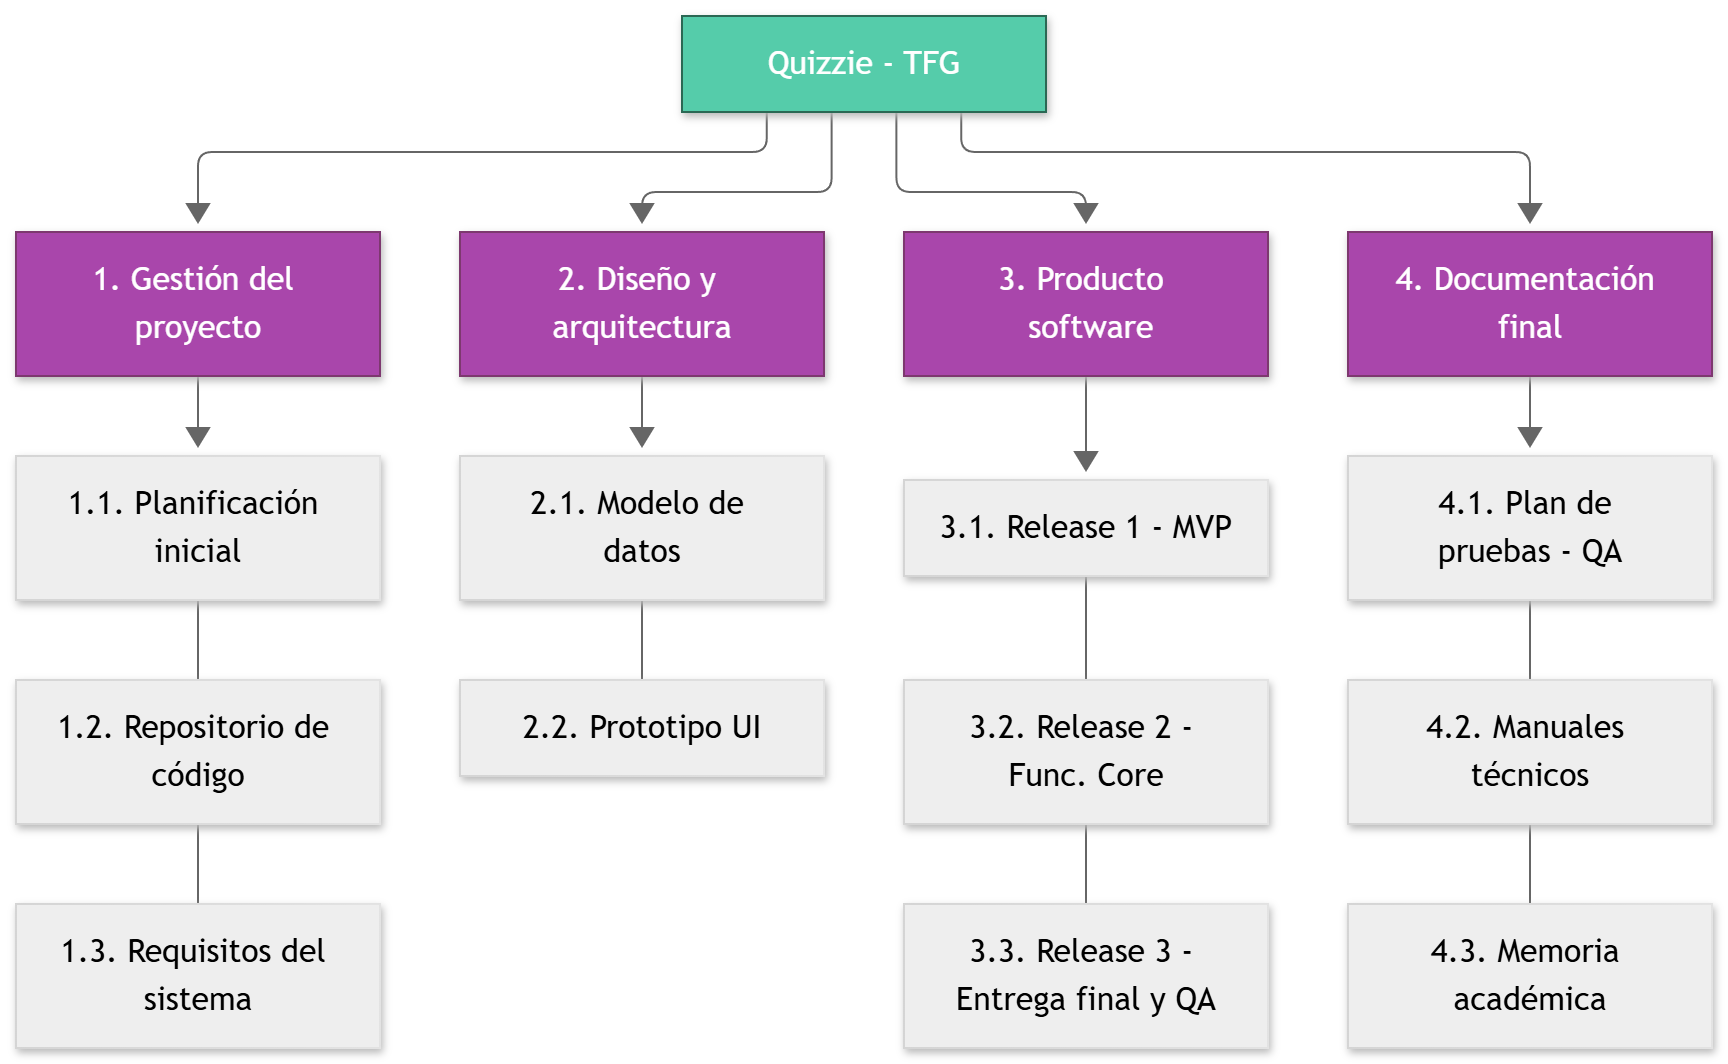
\includegraphics[width=0.87\textwidth]{figures/edt.png}
\caption{Estructura de Desglose del Trabajo (EDT).}
\label{fig:edt_grafica}
\end{figure}

Esta representación jerárquica descompone el proyecto en \textbf{paquetes de trabajo} y \textbf{entregables específicos} según las directrices de descomposición del estándar ISO/IEC/IEEE 21839 \cite{iso21839}, los cuales se detallan en el diccionario de la EDT.

\subsection{Diccionario de la EDT}\label{subsec:diccionario_edt}

El diccionario de la EDT define formalmente el \textbf{alcance} de cada entregable y desglosa las actividades necesarias para su consecución, especificando los perfiles profesionales asignados y la estimación temporal.

\subsubsection*{Paquete 1: Gestión del proyecto}
\addcontentsline{toc}{subsubsection}{Paquete 1: Gestión del proyecto}

\begin{table}[H]
\centering
\small
\renewcommand{\arraystretch}{1.2}
\makebox[\textwidth][c]{%
\begin{tabular}{P{3.3cm} P{5.8cm} @{}c@{}}
\bighline
\textbf{Entregable} & \textbf{Descripción} & 
\begin{tabular}{c c c}
  \makebox[2.2cm][c]{\textbf{Actividad}} & \makebox[2.3cm][c]{\textbf{Recurso}} & \makebox[1.2cm][c]{\textbf{Horas}}
\end{tabular} \\ \bighline

1.1. Planificación inicial & 
Acta de constitución del proyecto y cronograma base estimado para fijar los hitos académicos. & 
{%
  \renewcommand{\arraystretch}{1.2}
  \begin{tabular}[t]{>{\centering\arraybackslash}p{2.2cm} >{\centering\arraybackslash}p{2.3cm} >{\centering\arraybackslash}p{1.2cm}}
    \hyperref[act:01]{\textbf{ACT-01}} & Project Manager & 4h \\ \cmidrule(l{4pt}){1-3}
    \hyperref[act:02]{\textbf{ACT-02}} & Project Manager & 4h
  \end{tabular}%
} \\ \hline

1.2. Repositorio de código & 
Configuración de GitHub con reglas de protección de ramas, flujos de trabajo basados en fusiones (\textit{merges}) y plantillas estandarizadas para \textit{issues}. & 
{%
  \renewcommand{\arraystretch}{1.2}
  \begin{tabular}[t]{>{\centering\arraybackslash}p{2.2cm} >{\centering\arraybackslash}p{2.3cm} >{\centering\arraybackslash}p{1.2cm}}
    \hyperref[act:13]{\textbf{ACT-13}} & Técnico & 11h \\ \cmidrule(l{4pt}){1-3}
    \hyperref[act:14]{\textbf{ACT-14}} & Técnico & 5h \\ \cmidrule(l{4pt}){1-3}
    \hyperref[act:15]{\textbf{ACT-15}} & Técnico & 12h
  \end{tabular}%
} \\ \hline

1.3. Requisitos del sistema & 
Catálogo de requisitos funcionales y no funcionales, junto al modelado de casos de uso y flujos \textit{core} de la aplicación. & 
{%
  \renewcommand{\arraystretch}{1.2}
  \begin{tabular}[t]{>{\centering\arraybackslash}p{2.2cm} >{\centering\arraybackslash}p{2.3cm} >{\centering\arraybackslash}p{1.2cm}}
    \hyperref[act:08]{\textbf{ACT-08}} & Analista & 3h \\ \cmidrule(l{4pt}){1-3}
    \hyperref[act:09]{\textbf{ACT-09}} & Analista & 4h
  \end{tabular}%
} \\ \bighline
\end{tabular}%
}
\caption{Diccionario de la EDT - 1. Gestión del proyecto}
\label{tab:diccionario_edt_gestion_proyecto}
\end{table}

\subsubsection*{Paquete 2: Diseño y arquitectura}
\addcontentsline{toc}{subsubsection}{Paquete 2: Diseño y arquitectura}

\begin{table}[H]
\centering
\small
\renewcommand{\arraystretch}{1.2}
\makebox[\textwidth][c]{%
\begin{tabular}{P{3.3cm} P{5.8cm} @{}c@{}}
\bighline
\textbf{Entregable} & \textbf{Descripción} & 
\begin{tabular}{c c c}
  \makebox[2.2cm][c]{\textbf{Actividad}} & \makebox[2.3cm][c]{\textbf{Recurso}} & \makebox[1.2cm][c]{\textbf{Horas}}
\end{tabular} \\ \bighline

2.1. Modelo de datos & 
Diseño conceptual, lógico y físico de la base de datos relacional, materializado en el diagrama de entidades del sistema. & 
{%
  \renewcommand{\arraystretch}{1.2}
  \begin{tabular}[t]{>{\centering\arraybackslash}p{2.2cm} >{\centering\arraybackslash}p{2.3cm} >{\centering\arraybackslash}p{1.2cm}}
    \hyperref[act:10]{\textbf{ACT-10}} & Analista & 4h \\ \cmidrule(l{4pt}){1-3}
    \hyperref[act:11]{\textbf{ACT-11}} & Analista & 4h \\ \cmidrule(l{4pt}){1-3}
    \hyperref[act:12]{\textbf{ACT-12}} & Programador Backend & 2h
  \end{tabular}%
} \\ \hline

2.2. Prototipo UI & 
Diseños visuales y plantillas para las pantallas del sistema. & 
{%
  \renewcommand{\arraystretch}{1.2}
  \begin{tabular}[t]{>{\centering\arraybackslash}p{2.2cm} >{\centering\arraybackslash}p{2.3cm} >{\centering\arraybackslash}p{1.2cm}}
    \hyperref[act:03]{\textbf{ACT-03}} & Diseñador UI & 2h \\ \cmidrule(l{4pt}){1-3}
    \hyperref[act:04]{\textbf{ACT-04}} & Diseñador UI & 5h \\ \cmidrule(l{4pt}){1-3}
    \hyperref[act:05]{\textbf{ACT-05}} & Diseñador UI & 5h
  \end{tabular}%
} \\ \bighline
\end{tabular}%
}
\caption{Diccionario de la EDT - 2. Diseño y arquitectura}
\label{tab:diccionario_edt_diseno_arquitectura}
\end{table}

\subsubsection*{Paquete 3: Producto software}
\addcontentsline{toc}{subsubsection}{Paquete 3: Producto software}

\begin{table}[H]
\centering
\small
\renewcommand{\arraystretch}{1.2}
\makebox[\textwidth][c]{%
\begin{tabular}{P{3.3cm} P{5.8cm} @{}c@{}}
\bighline
\textbf{Entregable} & \textbf{Descripción} & 
\begin{tabular}{c c c}
  \makebox[2.2cm][c]{\textbf{Actividad}} & \makebox[2.3cm][c]{\textbf{Recurso}} & \makebox[1.2cm][c]{\textbf{Horas}}
\end{tabular} \\ \bighline

3.1. Release 1 (MVP) & 
Habilitación y despliegue del flujo completo base del sistema, permitiendo la creación de cuestionarios por parte del profesor y la realización de los mismos por los alumnos. & 
{%
  \renewcommand{\arraystretch}{1.2}
  \begin{tabular}[t]{>{\centering\arraybackslash}p{2.2cm} >{\centering\arraybackslash}p{2.3cm} >{\centering\arraybackslash}p{1.2cm}}
    \hyperref[act:16]{\textbf{ACT-16}} & Programador Backend & 25h \\ \cmidrule(l{4pt}){1-3}
    \hyperref[act:17]{\textbf{ACT-17}} & Programador Frontend & 25h \\ \cmidrule(l{4pt}){1-3}
    \hyperref[act:18]{\textbf{ACT-18}} & Programador Backend & 15h
  \end{tabular}%
} \\ \hline

3.2. Release 2 (Funcionalidades Core) & 
Implementación de la capa de comunicación en tiempo real mediante WebSockets y el motor de validación de datos del sistema. & 
{%
  \renewcommand{\arraystretch}{1.2}
  \begin{tabular}[t]{>{\centering\arraybackslash}p{2.2cm} >{\centering\arraybackslash}p{2.3cm} >{\centering\arraybackslash}p{1.2cm}}
    \hyperref[act:21]{\textbf{ACT-21}} & Programador Backend & 20h \\ \cmidrule(l{4pt}){1-3}
    \hyperref[act:22]{\textbf{ACT-22}} & Programador Frontend & 17h \\ \cmidrule(l{4pt}){1-3}
    \hyperref[act:23]{\textbf{ACT-23}} & Programador Backend & 12h
  \end{tabular}%
} \\ \hline

3.3. Release 3 (Entrega final y QA) & 
Integración de funcionalidades avanzadas de gestión, pulido general de la interfaz y despliegue del sistema. & 
{%
  \renewcommand{\arraystretch}{1.2}
  \begin{tabular}[t]{>{\centering\arraybackslash}p{2.2cm} >{\centering\arraybackslash}p{2.3cm} >{\centering\arraybackslash}p{1.2cm}}
    \hyperref[act:24]{\textbf{ACT-24}} & Programador Backend & 5h \\ \cmidrule(l{4pt}){1-3}
    \hyperref[act:25]{\textbf{ACT-25}} & Programador Frontend & 5h \\ \cmidrule(l{4pt}){1-3}
    \hyperref[act:26]{\textbf{ACT-26}} & Técnico & 3h
  \end{tabular}%
} \\ \bighline
\end{tabular}%
}
\caption{Diccionario de la EDT - 3. Producto software}
\label{tab:diccionario_edt_producto_software}
\end{table}

\subsubsection*{Paquete 4: Documentación final}
\addcontentsline{toc}{subsubsection}{Paquete 4: Documentación final}

\begin{table}[H]
\centering
\small
\renewcommand{\arraystretch}{1.2}
\makebox[\textwidth][c]{%
\begin{tabular}{P{3.3cm} P{5.8cm} @{}c@{}}
\bighline
\textbf{Entregable} & \textbf{Descripción} & 
\begin{tabular}{c c c}
  \makebox[2.2cm][c]{\textbf{Actividad}} & \makebox[2.3cm][c]{\textbf{Recurso}} & \makebox[1.2cm][c]{\textbf{Horas}}
\end{tabular} \\ \bighline

4.1. Plan de pruebas (QA) & 
Diseño y ejecución de baterías de test de integración y \textit{scripts} específicos de pruebas de carga. & 
{%
  \renewcommand{\arraystretch}{1.2}
  \begin{tabular}[t]{>{\centering\arraybackslash}p{2.2cm} >{\centering\arraybackslash}p{2.3cm} >{\centering\arraybackslash}p{1.2cm}}
    \hyperref[act:19]{\textbf{ACT-19}} & Tester & 7h \\ \cmidrule(l{4pt}){1-3}
    \hyperref[act:20]{\textbf{ACT-20}} & Tester & 8h
  \end{tabular}%
} \\ \hline

4.2. Manuales técnicos & 
Redacción del manual de usuario y del manual de despliegue. & 
{%
  \renewcommand{\arraystretch}{1.2}
  \begin{tabular}[t]{>{\centering\arraybackslash}p{2.2cm} >{\centering\arraybackslash}p{2.3cm} >{\centering\arraybackslash}p{1.2cm}}
    \hyperref[act:06]{\textbf{ACT-06}} & Analista & 2h \\ \cmidrule(l{4pt}){1-3}
    \hyperref[act:07]{\textbf{ACT-07}} & Técnico & 1h
  \end{tabular}%
} \\ \hline

4.3. Memoria académica & 
Redacción técnica, maquetación y consolidación del documento final del TFG junto con el diseño de las diapositivas para la defensa. & 
{%
  \renewcommand{\arraystretch}{1.2}
  \begin{tabular}[t]{>{\centering\arraybackslash}p{2.2cm} >{\centering\arraybackslash}p{2.3cm} >{\centering\arraybackslash}p{1.2cm}}
    \hyperref[act:27]{\textbf{ACT-27}} & Analista & 70h \\ \cmidrule(l{4pt}){1-3}
    \hyperref[act:28]{\textbf{ACT-28}} & Diseñador UI & 10h \\ \cmidrule(l{4pt}){1-3}
    \hyperref[act:29]{\textbf{ACT-29}} & Project Manager & 10h
  \end{tabular}%
} \\ \bighline
\end{tabular}%
}
\caption{Diccionario de la EDT - 4. Documentación final}
\label{tab:diccionario_edt_documentacion_final}
\end{table}


\section{Línea base del cronograma}\label{sec:linea_base_del_cronograma}
A partir de los paquetes de trabajo de la \hyperref[subsec:edt]{EDT}, se ha planificado la distribución temporal del proyecto. El flujo de trabajo se estructura dividiendo el ciclo de vida en fases temporales que agrupan las actividades y culminan en hitos de control.

\subsection{Fases del proyecto}\label{sub:fases_del_proyecto}

El proyecto se divide en 10 fases temporales consecutivas y paralelas, que se han organizado en 4 bloques de trabajo fundamentales:

\begin{table}[H]
\centering
\small
\renewcommand{\arraystretch}{1.4}
\makebox[\textwidth][c]{%
\begin{tabularx}{1\textwidth}{llYl}
\bighline
\textbf{ID} &  \textbf{Nombre} & \textbf{Descripción} & \textbf{Bloque} \\ \bighline
F-01 & Planificación & Planificación inicial, estimación de tiempos y recursos. & Gestión y planificación \\ \hline
F-02 & Documentación & Redacción de manuales y documentación técnica de soporte. & Documentación y cierre \\ \hline
F-03 & Inicio & Configuración del entorno base y análisis de requisitos. & Gestión y planificación \\ \hline
F-04 & CI/CD & Automatización de flujos de trabajo e integración continua. & Ciclo de vida y calidad \\ \hline
F-05 \label{fase:mvp} & MVP & Construcción de la primera versión mínima funcional. & Desarrollo de código \\ \hline
F-06 & Testing & Diseño y ejecución de la batería de pruebas del sistema. & Ciclo de vida y calidad \\ \hline
F-07 \label{fase:core} & Core & Desarrollo de las características principales (WebSockets). & Desarrollo de código \\ \hline
F-08 \label{fase:qa} & QA & Estabilización de código y corrección de errores finales. & Desarrollo de código \\ \hline
F-09 & Memoria & Consolidación, revisión final y entrega de la memoria. & Documentación y cierre \\ \hline
F-10 & Defensa & Preparación del material de soporte y ensayos. & Documentación y cierre \\ \bighline
\end{tabularx}%
}
\caption{Fases temporales del proyecto.}
\label{tab:fases}
\end{table}

\subsection{Lista de actividades}\label{sub:lista_de_actividades}

Cada una de las actividades del cronograma conserva una relación directa con los paquetes de trabajo definidos en el diccionario de la EDT. Para garantizar el seguimiento y la trazabilidad temporal, a continuación se detallan todas las tareas del proyecto:

\begin{table}[H]
\centering
\small
\renewcommand{\arraystretch}{1.48}
\makebox[\textwidth][c]{%
\begin{tabularx}{1.1\textwidth}{llY}
\bighline
\textbf{Fase} & \textbf{ID} & \textbf{Actividad} \\ \bighline

F-01 -- Planificación & ACT-01\label{act:01} & Redacción del acta de constitución \\ \cline{2-3}
& ACT-02\label{act:02} & Definición de hitos y estimación del cronograma inicial \\ \cline{2-3}
& ACT-03\label{act:03} & Elección de estilos, paleta de colores y componentes básicos \\ \cline{2-3}
& ACT-04\label{act:04} & Diseño de prototipos de las pantallas de gestión del profesor \\ \cline{2-3}
& ACT-05\label{act:05} & Diseño de la interfaz de respuesta para pantallas de alumnos \\ \hline

F-02 -- Documentación & ACT-06\label{act:06} & Elaboración del manual funcional como guía para usuarios \\ \cline{2-3}
& ACT-07\label{act:07} & Redacción del manual de despliegue técnico de infraestructura \\ \cline{2-3}
& ACT-08\label{act:08} & Elicitación y redacción de requisitos funcionales y no funcionales \\ \cline{2-3}
& ACT-09\label{act:09} & Modelado de diagramas de casos de uso y flujos esenciales \\ \cline{2-3}
& ACT-10\label{act:10} & Diseño del modelo conceptual y lógico de datos \\ \cline{2-3}
& ACT-11\label{act:11} & Modelado del diagrama de entidades relacional \\ \cline{2-3}
& ACT-12\label{act:12} & Generación del \textit{script} de inicialización de tablas y poblado \\ \hline

F-03 -- Inicio & ACT-13\label{act:13} & Inicialización del repositorio en GitHub y estructura base \\ \hline

F-04 -- CI/CD & ACT-14\label{act:14} & Diseño de \textit{templates} para \textit{issues} y automatización base \\ \cline{2-3}
& ACT-15\label{act:15} & Desarrollo de \textit{scripts} de despliegue e integración continuos \\ \hline

F-05 -- MVP & ACT-16\label{act:16} & Diseño y desarrollo de la persistencia base para cuestionarios \\ \cline{2-3}
& ACT-17\label{act:17} & Implementación de la interfaz de creación de tests y panel base \\ \cline{2-3}
& ACT-18\label{act:18} & Lógica de control y validación para la ejecución asíncrona \\ \hline

F-06 -- Testing & ACT-19\label{act:19} & Desarrollo y ejecución de test de integración de servicios \\ \cline{2-3}
& ACT-20\label{act:20} & Pruebas de componentes, de carga y \textit{end-to-end} \\ \hline

F-07 -- Core & ACT-21\label{act:21} & Desarrollo de la infraestructura síncrona y canales WebSocket \\ \cline{2-3}
& ACT-22\label{act:22} & Implementación en frontend de la conexión reactiva a salas \\ \cline{2-3}
& ACT-23\label{act:23} & Programación del motor de validación y control de integridad \\ \hline

F-08 -- QA & ACT-24\label{act:24} & Implementación del módulo de autenticación y panel avanzado \\ \cline{2-3}
& ACT-25\label{act:25} & Desarrollo de vistas de historial y exportación de datos \\ \cline{2-3}
& ACT-26\label{act:26} & Puesta a punto, empaquetado, corrección de errores y despliegue \\ \hline

F-09 -- Memoria & ACT-27\label{act:27} & Redacción y estructuración técnica de la memoria en LaTeX \\ \hline

F-10 -- Defensa & ACT-28\label{act:28} & Diseño, desarrollo y maquetación de diapositivas de defensa \\ \cline{2-3}
& ACT-29\label{act:29} & Ensayos de oratoria y preparación de la defensa pública \\ \bighline
\end{tabularx}%
}
\caption{Actividades organizadas por su fase del cronograma.}
\label{tab:lista_actividades}
\end{table}

\subsection{Lista de hitos}\label{sub:lista_de_hitos}

Los hitos representan los puntos de control clave y logros de duración cero dentro del cronograma del proyecto. Su consecución suponen grandes avances en el desarrollo o la finalización de fases completas, y permiten evaluar el progreso general del proyecto. 

\begin{table}[H]
\centering
\small
\renewcommand{\arraystretch}{1.6}
\makebox[\textwidth][c]{%
\begin{tabularx}{1\textwidth}{llYc}
\bighline
\textbf{Fase} & \textbf{ID} & \textbf{Hito / logro} & \textbf{Límite} \\ \bighline

F-01 -- Planificación & H-01 & Acta de constitución del proyecto redactada y firmada & 21 Ene \\ \cline{2-4}
& H-02 & Líneas base del proyecto constituidas y aprobadas & 28 Ene \\ \hline

F-02 -- Documentación & H-03 & Catálogo de requisitos, casos de uso y modelos de datos definidos & 18 Feb \\ \cline{2-4}
& H-04 & Manuales técnicos de usuario y despliegue finalizados & 14 Abr \\ \hline

F-03 -- Inicio & H-05 & Repositorio inicializado y entorno de desarrollo listo & 11 Feb \\ \hline

F-04 -- CI/CD & H-06 & Flujo de CI/CD automatizado y plantillas de trabajo desplegadas & 1 Mar \\ \hline

F-05 -- MVP & H-07 & Funcionalidades del MVP operativas (creación y respuesta de tests) & 8 Mar \\ \hline

F-06 -- Testing & H-08 & Baterías de pruebas de software ejecutadas y superadas con éxito & 26 Abr \\ \hline

F-07 -- Core & H-09 & Conexión y respuesta a cuestionarios en tiempo real operativos & 29 Mar \\ \cline{2-4}
& H-10 & Motor de validación y control de integridad de respuestas completado & 12 Abr \\ \hline

F-08 -- QA & H-11 & Vistas de historial de salas pasadas y exportación de datos funcionales & 24 Abr \\ \hline

F-09 -- Memoria & H-12 & Memoria académica consolidada y entregada & 17 May \\ \hline

F-10 -- Defensa & H-13 & Presentación y material de soporte maquetados para la defensa & 5 Jun \\ \cline{2-4}
& H-14 & Defensa pública del proyecto ejecutada ante el tribunal & 10 Jun \\ \bighline
\end{tabularx}%
}
\caption{Hitos de control del proyecto.}
\label{tab:lista_hitos}
\end{table}


\subsection{Diagrama de Gantt}\label{sub:diagrama_de_gantt}
El siguiente diagrama de Gantt\cite{wilson2003gantt} sintetiza de manera visual la distribución cronológica del proyecto, clave para el seguimiento del trabajo realizado y asegurar el cumplimiento de los plazos fijados.

\begin{figure}[H]
\centering
\makebox[\textwidth][c]{
\begin{ganttchart}[
    hgrid=false, 
    vgrid=false, 
    x unit=0.115cm,
    y unit title=0.65cm, 
    y unit chart=0.95cm, 
    bar height=0.55,
    time slot format=isodate,
    inline,
    bar label font=\small\bfseries\color{white},
    ganttbar label node/.style={text width=0pt, inner sep=0pt},
    title label font=\small\bfseries,
    title calendar link/.style={draw=black},
    canvas/.style={draw=black, fill=white}
]{2026-01-15}{2026-06-12}

    % Única fila de meses
    \gantttitle{Ene}{17}
    \gantttitle{Feb}{28}
    \gantttitle{Mar}{31}
    \gantttitle{Abr}{30}
    \gantttitle{May}{31}
    \gantttitle{Jun}{12} \\

    % Fases
    \ganttbar[bar/.style={fill=primaryMagenta, draw=primaryMagenta, rounded corners=2.5pt}]{F01-Plan}{2026-01-15}{2026-01-28} \\
    \ganttbar[bar/.style={fill=secondaryMagenta, draw=secondaryMagenta, rounded corners=2.5pt}]{F02-Documentación}{2026-01-29}{2026-04-14} \\
    \ganttbar[bar/.style={fill=primaryMagenta, draw=primaryMagenta, rounded corners=2.5pt}]{F03-Inicio}{2026-01-29}{2026-02-11} \\
    \ganttbar[bar/.style={fill=secondaryCyan, draw=secondaryCyan, rounded corners=2.5pt}]{F04-CI/CD}{2026-02-12}{2026-04-26} \\
    \ganttbar[bar/.style={fill=primaryCyan, draw=primaryCyan, rounded corners=2.5pt}]{F05-MVP}{2026-02-19}{2026-03-08} \\
    \ganttbar[bar/.style={fill=secondaryCyan, draw=secondaryCyan, rounded corners=2.5pt}]{F06-Testing}{2026-02-24}{2026-04-26} \\
    \ganttbar[bar/.style={fill=primaryCyan, draw=primaryCyan, rounded corners=2.5pt}]{F07-Core}{2026-03-09}{2026-04-12} \\
    \ganttbar[bar/.style={fill=primaryCyan, draw=primaryCyan, rounded corners=2.5pt}]{F08-QA}{2026-04-13}{2026-04-24} \\
    \ganttbar[bar/.style={fill=secondaryMagenta, draw=secondaryMagenta, rounded corners=2.5pt}]{F09-Memoria}{2026-04-15}{2026-05-17} \\
    \ganttbar[bar/.style={fill=secondaryMagenta, draw=secondaryMagenta, rounded corners=2.5pt}]{F10-Defensa}{2026-05-18}{2026-06-12} \\
    % Espacio inferior para holgura de hitos
    \ganttbar[bar/.style={draw=none, fill=none}]{}{2026-01-15}{2026-01-15}

    \begin{pgfonlayer}{behind}
        
        % 1.1 Líneas semanales 
        \ganttvrule[vrule/.style={draw=gray!70, densely dotted, thick}]{}{2026-01-19}
        \ganttvrule[vrule/.style={draw=gray!70, densely dotted, thick}]{}{2026-01-26}
        \ganttvrule[vrule/.style={draw=gray!70, densely dotted, thick}]{}{2026-02-02}
        \ganttvrule[vrule/.style={draw=gray!70, densely dotted, thick}]{}{2026-02-09}
        \ganttvrule[vrule/.style={draw=gray!70, densely dotted, thick}]{}{2026-02-16}
        \ganttvrule[vrule/.style={draw=gray!70, densely dotted, thick}]{}{2026-02-23}
        \ganttvrule[vrule/.style={draw=gray!70, densely dotted, thick}]{}{2026-03-02}
        \ganttvrule[vrule/.style={draw=gray!70, densely dotted, thick}]{}{2026-03-09}
        \ganttvrule[vrule/.style={draw=gray!70, densely dotted, thick}]{}{2026-03-16}
        \ganttvrule[vrule/.style={draw=gray!70, densely dotted, thick}]{}{2026-03-23}
        \ganttvrule[vrule/.style={draw=gray!70, densely dotted, thick}]{}{2026-03-30}
        \ganttvrule[vrule/.style={draw=gray!70, densely dotted, thick}]{}{2026-04-06}
        \ganttvrule[vrule/.style={draw=gray!70, densely dotted, thick}]{}{2026-04-13}
        \ganttvrule[vrule/.style={draw=gray!70, densely dotted, thick}]{}{2026-04-20}
        \ganttvrule[vrule/.style={draw=gray!70, densely dotted, thick}]{}{2026-04-27}
        \ganttvrule[vrule/.style={draw=gray!70, densely dotted, thick}]{}{2026-05-04}
        \ganttvrule[vrule/.style={draw=gray!70, densely dotted, thick}]{}{2026-05-11}
        \ganttvrule[vrule/.style={draw=gray!70, densely dotted, thick}]{}{2026-05-18}
        \ganttvrule[vrule/.style={draw=gray!70, densely dotted, thick}]{}{2026-05-25}
        \ganttvrule[vrule/.style={draw=gray!70, densely dotted, thick}]{}{2026-06-01}
        \ganttvrule[vrule/.style={draw=gray!70, densely dotted, thick}]{}{2026-06-08}

        % 1.2 Líneas verticales discontinuas de los hitos
        \ganttvrule[vrule/.style={draw=primaryMagenta, dashed, line width=1.3pt}]{}{2026-01-21}
        \ganttvrule[vrule/.style={draw=primaryMagenta, dashed, line width=1.3pt}]{}{2026-01-28}
        \ganttvrule[vrule/.style={draw=primaryMagenta, dashed, line width=1.3pt}]{}{2026-02-11}
        \ganttvrule[vrule/.style={draw=primaryCyan, dashed, line width=1.3pt}]{}{2026-03-08}
        \ganttvrule[vrule/.style={draw=primaryCyan, dashed, line width=1.3pt}]{}{2026-03-29}
        \ganttvrule[vrule/.style={draw=primaryCyan, dashed, line width=1.3pt}]{}{2026-04-12}
        \ganttvrule[vrule/.style={draw=primaryCyan, dashed, line width=1.3pt}]{}{2026-04-24}
        \ganttvrule[vrule/.style={draw=secondaryCyan, dashed, line width=1.3pt}]{}{2026-03-01}
        \ganttvrule[vrule/.style={draw=secondaryCyan, dashed, line width=1.3pt}]{}{2026-04-26}
        \ganttvrule[vrule/.style={draw=secondaryMagenta, dashed, line width=1.3pt}]{}{2026-02-18}
        \ganttvrule[vrule/.style={draw=secondaryMagenta, dashed, line width=1.3pt}]{}{2026-04-14}
        \ganttvrule[vrule/.style={draw=secondaryMagenta, dashed, line width=1.3pt}]{}{2026-05-17}
        \ganttvrule[vrule/.style={draw=secondaryMagenta, dashed, line width=1.3pt}]{}{2026-06-05}
        \ganttvrule[vrule/.style={draw=secondaryMagenta, dashed, line width=1.3pt}]{}{2026-06-10}

    
        % 2.1 Números semanales superiores con fondo blanco
        \ganttvrule[vrule/.style={draw=none}, vrule label node/.style={at end, anchor=north, yshift=305pt, font=\small\bfseries\color{gray!90!black}, fill=white, inner sep=2pt, rounded corners=1pt}]{19}{2026-01-19}
        \ganttvrule[vrule/.style={draw=none}, vrule label node/.style={at end, anchor=north, yshift=305pt, font=\small\bfseries\color{gray!90!black}, fill=white, inner sep=2pt, rounded corners=1pt}]{26}{2026-01-26}
        \ganttvrule[vrule/.style={draw=none}, vrule label node/.style={at end, anchor=north, yshift=305pt, font=\small\bfseries\color{gray!90!black}, fill=white, inner sep=2pt, rounded corners=1pt}]{02}{2026-02-02}
        \ganttvrule[vrule/.style={draw=none}, vrule label node/.style={at end, anchor=north, yshift=305pt, font=\small\bfseries\color{gray!90!black}, fill=white, inner sep=2pt, rounded corners=1pt}]{09}{2026-02-09}
        \ganttvrule[vrule/.style={draw=none}, vrule label node/.style={at end, anchor=north, yshift=305pt, font=\small\bfseries\color{gray!90!black}, fill=white, inner sep=2pt, rounded corners=1pt}]{16}{2026-02-16}
        \ganttvrule[vrule/.style={draw=none}, vrule label node/.style={at end, anchor=north, yshift=305pt, font=\small\bfseries\color{gray!90!black}, fill=white, inner sep=2pt, rounded corners=1pt}]{23}{2026-02-23}
        \ganttvrule[vrule/.style={draw=none}, vrule label node/.style={at end, anchor=north, yshift=305pt, font=\small\bfseries\color{gray!90!black}, fill=white, inner sep=2pt, rounded corners=1pt}]{02}{2026-03-02}
        \ganttvrule[vrule/.style={draw=none}, vrule label node/.style={at end, anchor=north, yshift=305pt, font=\small\bfseries\color{gray!90!black}, fill=white, inner sep=2pt, rounded corners=1pt}]{09}{2026-03-09}
        \ganttvrule[vrule/.style={draw=none}, vrule label node/.style={at end, anchor=north, yshift=305pt, font=\small\bfseries\color{gray!90!black}, fill=white, inner sep=2pt, rounded corners=1pt}]{16}{2026-03-16}
        \ganttvrule[vrule/.style={draw=none}, vrule label node/.style={at end, anchor=north, yshift=305pt, font=\small\bfseries\color{gray!90!black}, fill=white, inner sep=2pt, rounded corners=1pt}]{23}{2026-03-23}
        \ganttvrule[vrule/.style={draw=none}, vrule label node/.style={at end, anchor=north, yshift=305pt, font=\small\bfseries\color{gray!90!black}, fill=white, inner sep=2pt, rounded corners=1pt}]{30}{2026-03-30}
        \ganttvrule[vrule/.style={draw=none}, vrule label node/.style={at end, anchor=north, yshift=305pt, font=\small\bfseries\color{gray!90!black}, fill=white, inner sep=2pt, rounded corners=1pt}]{06}{2026-04-06}
        \ganttvrule[vrule/.style={draw=none}, vrule label node/.style={at end, anchor=north, yshift=305pt, font=\small\bfseries\color{gray!90!black}, fill=white, inner sep=2pt, rounded corners=1pt}]{13}{2026-04-13}
        \ganttvrule[vrule/.style={draw=none}, vrule label node/.style={at end, anchor=north, yshift=305pt, font=\small\bfseries\color{gray!90!black}, fill=white, inner sep=2pt, rounded corners=1pt}]{20}{2026-04-20}
        \ganttvrule[vrule/.style={draw=none}, vrule label node/.style={at end, anchor=north, yshift=305pt, font=\small\bfseries\color{gray!90!black}, fill=white, inner sep=2pt, rounded corners=1pt}]{27}{2026-04-27}
        \ganttvrule[vrule/.style={draw=none}, vrule label node/.style={at end, anchor=north, yshift=305pt, font=\small\bfseries\color{gray!90!black}, fill=white, inner sep=2pt, rounded corners=1pt}]{04}{2026-05-04}
        \ganttvrule[vrule/.style={draw=none}, vrule label node/.style={at end, anchor=north, yshift=305pt, font=\small\bfseries\color{gray!90!black}, fill=white, inner sep=2pt, rounded corners=1pt}]{11}{2026-05-11}
        \ganttvrule[vrule/.style={draw=none}, vrule label node/.style={at end, anchor=north, yshift=305pt, font=\small\bfseries\color{gray!90!black}, fill=white, inner sep=2pt, rounded corners=1pt}]{18}{2026-05-18}
        \ganttvrule[vrule/.style={draw=none}, vrule label node/.style={at end, anchor=north, yshift=305pt, font=\small\bfseries\color{gray!90!black}, fill=white, inner sep=2pt, rounded corners=1pt}]{25}{2026-05-25}
        \ganttvrule[vrule/.style={draw=none}, vrule label node/.style={at end, anchor=north, yshift=305pt, font=\small\bfseries\color{gray!90!black}, fill=white, inner sep=2pt, rounded corners=1pt}]{01}{2026-06-01}
        \ganttvrule[vrule/.style={draw=none}, vrule label node/.style={at end, anchor=north, yshift=305pt, font=\small\bfseries\color{gray!90!black}, fill=white, inner sep=2pt, rounded corners=1pt}]{08}{2026-06-08}

        % 2.2 Etiquetas de hitos 
        % Gestión y planificación
        \ganttvrule[vrule/.style={draw=none}, vrule label node/.style={anchor=south, yshift=4pt, font=\small\bfseries\color{primaryMagenta}, fill=white, inner sep=2pt, rounded corners=1pt}]{H-01}{2026-01-21}
        \ganttvrule[vrule/.style={draw=none}, vrule label node/.style={anchor=south, yshift=0.55cm, font=\small\bfseries\color{primaryMagenta}, fill=white, inner sep=2pt, rounded corners=1pt}]{H-02}{2026-01-28}
        \ganttvrule[vrule/.style={draw=none}, vrule label node/.style={anchor=south, yshift=4pt, font=\small\bfseries\color{primaryMagenta}, fill=white, inner sep=2pt, rounded corners=1pt}]{H-05}{2026-02-11}

        % Desarrollo de código
        \ganttvrule[vrule/.style={draw=none}, vrule label node/.style={anchor=south, yshift=0.55cm, font=\small\bfseries\color{primaryCyan}, fill=white, inner sep=2pt, rounded corners=1pt}]{H-07}{2026-03-08}
        \ganttvrule[vrule/.style={draw=none}, vrule label node/.style={anchor=south, yshift=4pt, font=\small\bfseries\color{primaryCyan}, fill=white, inner sep=2pt, rounded corners=1pt}]{H-09}{2026-03-29}
        \ganttvrule[vrule/.style={draw=none}, vrule label node/.style={anchor=south, yshift=4pt, font=\small\bfseries\color{primaryCyan}, fill=white, inner sep=2pt, rounded corners=1pt}]{H-10}{2026-04-12}
        \ganttvrule[vrule/.style={draw=none}, vrule label node/.style={anchor=south, yshift=4pt, font=\small\bfseries\color{primaryCyan}, fill=white, inner sep=2pt, rounded corners=1pt}]{H-11}{2026-04-24}

        % Ciclo de vida y calidad
        \ganttvrule[vrule/.style={draw=none}, vrule label node/.style={anchor=south, yshift=4pt, font=\small\bfseries\color{secondaryCyan}, fill=white, inner sep=2pt, rounded corners=1pt}]{H-06}{2026-03-01}
        \ganttvrule[vrule/.style={draw=none}, vrule label node/.style={anchor=south, yshift=0.55cm, font=\small\bfseries\color{secondaryCyan}, fill=white, inner sep=2pt, rounded corners=1pt}]{H-08}{2026-04-26}

        % Documentación y cierre
        \ganttvrule[vrule/.style={draw=none}, vrule label node/.style={anchor=south, yshift=0.55cm, font=\small\bfseries\color{secondaryMagenta}, fill=white, inner sep=2pt, rounded corners=1pt}]{H-03}{2026-02-18}
        \ganttvrule[vrule/.style={draw=none}, vrule label node/.style={anchor=south, yshift=0.55cm, font=\small\bfseries\color{secondaryMagenta}, fill=white, inner sep=2pt, rounded corners=1pt}]{H-04}{2026-04-14}
        \ganttvrule[vrule/.style={draw=none}, vrule label node/.style={anchor=south, yshift=4pt, font=\small\bfseries\color{secondaryMagenta}, fill=white, inner sep=2pt, rounded corners=1pt}]{H-12}{2026-05-17}
        \ganttvrule[vrule/.style={draw=none}, vrule label node/.style={anchor=south, yshift=0.55cm, font=\small\bfseries\color{secondaryMagenta}, fill=white, inner sep=2pt, rounded corners=1pt}]{H-13}{2026-06-05}
        \ganttvrule[vrule/.style={draw=none}, vrule label node/.style={anchor=south, yshift=4pt, font=\small\bfseries\color{secondaryMagenta}, fill=white, inner sep=2pt, rounded corners=1pt}]{H-14}{2026-06-10}
    \end{pgfonlayer}

\end{ganttchart}
}
\vspace{0.25cm}
\begin{center}
\small
\begin{tabular}{clccl}
\fcolorbox{black}{primaryMagenta}{\rule{0pt}{4pt}\rule{4pt}{0pt}} & Gestión y planificación & \hspace{0.5cm} &
\fcolorbox{black}{primaryCyan}{\rule{0pt}{4pt}\rule{4pt}{0pt}} & Desarrollo de código \\
\fcolorbox{black}{secondaryCyan}{\rule{0pt}{4pt}\rule{4pt}{0pt}} & Ciclo de vida y calidad & \hspace{0.5cm} &
\fcolorbox{black}{secondaryMagenta}{\rule{0pt}{4pt}\rule{4pt}{0pt}} & Documentación y cierre
\end{tabular}
\end{center}
\caption{Diagrama de Gantt inicial del proyecto.}
\label{fig:gantt}
\end{figure}

\section{Línea base de Costes}\label{sec:linea_base_de_costes}
El desarrollo de un proyecto como \textit{Quizzie} no solo exige viabilidad técnica, sino también un \textbf{modelo financiero sostenible} que justifique su implantación frente a otras soluciones. Para ello, se analizan a continuación los costes operativos, el impacto económico que supone el escalado de la infraestructura y el Coste Total de Propiedad (TCO).

\subsection{Análisis de costes}\label{sub:analisis_de_costes}
El estudio económico de la plataforma se fundamenta en la clasificación financiera de costes de tecnologías de la información \cite{remenyi2007it}, dividiéndose en dos componentes esenciales: los Gastos de Capital (\textit{Capital Expenditure} o \textbf{CAPEX}), que engloban el coste de desarrollo y los recursos fijos iniciales, y los Gastos Operativos (\textit{Operational Expenditure} o \textbf{OPEX}), que representan el coste recurrente de la infraestructura en la nube para la explotación en producción.

\begin{table}[H]
\centering
\small
\renewcommand{\arraystretch}{1.4}
\makebox[\textwidth][c]{%
\begin{tabularx}{0.9\textwidth}{Yr}
\bighline
\textbf{Concepto} & \textbf{Coste neto} \\ \bighline
Costes laborales & 11.552,65 \euro \\ \hline
Equipamiento informático & 500,00 \euro \\ \hline
Licencia comercial anual Google AI Premium (Gemini Pro) & 218,07 \euro \\ \hline
Licencia GitHub Team (6 meses) & 21,82 \euro \\ \hline
Licencia Microsoft Teams Essentials (6 meses) & 21,82 \euro \\ \hline
Reserva de contingencia & 12.314,36 \euro \\ \bighline
\textbf{Total CAPEX} & \textbf{13.545,80 \euro} \\ \bighline
\end{tabularx}%
}
\caption{Resumen de Gastos de Capital (CAPEX).}
\label{tab:resumen_capex}
\end{table}

Para justificar el coste laboral del CAPEX, se adopta un \textbf{modelo de roles mixtos} debido a que el proyecto ha sido ejecutado íntegramente por un único ingeniero. De este modo, cada actividad de la EDT se presupuesta en función del perfil profesional específico requerido para su ejecución técnica.

Con el fin de garantizar el rigor y la objetividad de las tarifas aplicadas, los precios base por hora se han extraído del \textit{Informe Final sobre la Consulta Preliminar del Mercado: ``Perfiles Profesionales Ámbito Informático''} de la Junta de Andalucía \cite{juntaTIC2018}. Siguiendo las directrices de dicho organismo, se utiliza como referencia la \textbf{media acotada}, métrica estadística que descarta valores atípicos del sector mediante el test de Tukey.

Sobre la base salarial neta resultante de 8.886,65 \euro, se ha aplicado un \textbf{recargo del 30\%} en concepto de cotizaciones a la Seguridad Social y costes de contratación directos, consolidando el coste laboral real en \textbf{11.552,65 \euro}. El desglose detallado de horas y perfiles profesionales que sustenta este cálculo se recoge en la siguiente tabla de costes netos laborales.

\begin{table}[H]
\centering
\small
\renewcommand{\arraystretch}{1.2}
\makebox[\textwidth][c]{%
\begin{tabularx}{0.9\textwidth}{Ycccc}
\bighline
\textbf{Recurso (Rol)} & \textbf{Actividad} & \textbf{Precio/hora} & \textbf{Horas} & \textbf{Coste neto} \\ \bighline
\textbf{Project Manager}     & \hyperref[act:01]{\textbf{ACT-01}} & 46,09 \euro & 4 h  & 184,36 \euro \\ \cline{2-5}
                             & \hyperref[act:02]{\textbf{ACT-02}} & 46,09 \euro & 4 h  & 184,36 \euro \\ \cline{2-5}
                             & \hyperref[act:29]{\textbf{ACT-29}} & 46,09 \euro & 10 h & 460,90 \euro \\ \bigcline{2-5}
                         & \multicolumn{2}{l}{\textbf{Subtotal}}        & \textbf{18 h} & \textbf{829,62 \euro} \\ \hline
\textbf{Analista}            & \hyperref[act:06]{\textbf{ACT-06}} & 38,33 \euro & 2 h  & 76,66 \euro \\ \cline{2-5}
                             & \hyperref[act:08]{\textbf{ACT-08}} & 38,33 \euro & 3 h  & 114,99 \euro \\ \cline{2-5}
                             & \hyperref[act:09]{\textbf{ACT-09}} & 38,33 \euro & 4 h  & 153,32 \euro \\ \cline{2-5}
                             & \hyperref[act:10]{\textbf{ACT-10}} & 38,33 \euro & 4 h  & 153,32 \euro \\ \cline{2-5}
                             & \hyperref[act:11]{\textbf{ACT-11}} & 38,33 \euro & 4 h  & 153,32 \euro \\ \cline{2-5}
                             & \hyperref[act:27]{\textbf{ACT-27}} & 38,33 \euro & 70 h & 2.683,10 \euro \\ \bigcline{2-5}
                         & \multicolumn{2}{l}{\textbf{Subtotal}}        & \textbf{87 h} & \textbf{3.334,71 \euro} \\ \hline
\textbf{Diseñador UI}        & \hyperref[act:03]{\textbf{ACT-03}} & 33,43 \euro & 2 h  & 66,86 \euro \\ \cline{2-5}
                             & \hyperref[act:04]{\textbf{ACT-04}} & 33,43 \euro & 5 h  & 167,15 \euro \\ \cline{2-5}
                             & \hyperref[act:05]{\textbf{ACT-05}} & 33,43 \euro & 5 h  & 167,15 \euro \\ \cline{2-5}
                             & \hyperref[act:28]{\textbf{ACT-28}} & 33,43 \euro & 10 h & 334,30 \euro \\ \bigcline{2-5}
                         & \multicolumn{2}{l}{\textbf{Subtotal}}        & \textbf{22 h} & \textbf{735,46 \euro} \\ \hline
\textbf{Programador Backend} & \hyperref[act:12]{\textbf{ACT-12}} & 23,85 \euro & 2 h  & 47,70 \euro \\ \cline{2-5}
                             & \hyperref[act:16]{\textbf{ACT-16}} & 23,85 \euro & 25 h & 596,25 \euro \\ \cline{2-5}
                             & \hyperref[act:18]{\textbf{ACT-18}} & 23,85 \euro & 15 h  & 357,75 \euro \\ \cline{2-5}
                             & \hyperref[act:21]{\textbf{ACT-21}} & 23,85 \euro & 20 h & 477,00 \euro \\ \cline{2-5}
                             & \hyperref[act:23]{\textbf{ACT-23}} & 23,85 \euro & 12 h & 286,20 \euro \\ \cline{2-5}
                             & \hyperref[act:24]{\textbf{ACT-24}} & 23,85 \euro & 5 h  & 119,25 \euro \\ \bigcline{2-5}
                         & \multicolumn{2}{l}{\textbf{Subtotal}}        & \textbf{79 h} & \textbf{1.884,15 \euro} \\ \hline
\textbf{Programador Frontend} & \hyperref[act:17]{\textbf{ACT-17}} & 23,85 \euro & 25 h & 596,25 \euro \\ \cline{2-5}
                             & \hyperref[act:22]{\textbf{ACT-22}} & 23,85 \euro & 17 h & 405,45 \euro \\ \cline{2-5}
                             & \hyperref[act:25]{\textbf{ACT-25}} & 23,85 \euro & 5 h  & 119,25 \euro \\ \bigcline{2-5}
                         & \multicolumn{2}{l}{\textbf{Subtotal}}        & \textbf{47 h} & \textbf{1.120,95 \euro} \\ \hline
\textbf{Tester}              & \hyperref[act:19]{\textbf{ACT-19}} & 23,68 \euro & 7 h  & 165,76 \euro \\ \cline{2-5}
                             & \hyperref[act:20]{\textbf{ACT-20}} & 23,68 \euro & 8 h  & 189,44 \euro \\ \bigcline{2-5}
                         & \multicolumn{2}{l}{\textbf{Subtotal}}        & \textbf{15 h} & \textbf{355,20 \euro} \\ \hline
\textbf{Técnico}             & \hyperref[act:07]{\textbf{ACT-07}} & 19,58 \euro & 1 h  & 19,58 \euro \\ \cline{2-5}
                             & \hyperref[act:13]{\textbf{ACT-13}} & 19,58 \euro & 11 h & 215,38 \euro \\ \cline{2-5}
                             & \hyperref[act:14]{\textbf{ACT-14}} & 19,58 \euro & 5 h  & 97,90 \euro \\ \cline{2-5}
                             & \hyperref[act:15]{\textbf{ACT-15}} & 19,58 \euro & 12 h & 234,96 \euro \\ \cline{2-5}
                             & \hyperref[act:26]{\textbf{ACT-26}} & 19,58 \euro & 3 h  & 58,74 \euro \\ \bigcline{2-5}
                         & \multicolumn{2}{l}{\textbf{Subtotal}}        & \textbf{32 h} & \textbf{626,56 \euro} \\ \bighline
\textbf{TOTAL}         &   &   & \textbf{300 h} & \textbf{8.886,65 \euro} \\ \bighline
\end{tabularx}%
}
\caption{Costes netos laborales agrupados por perfil profesional.}
\label{tab:coste_personal_rol}
\end{table}

Una vez cuantificada la base de la mano de obra directa y consolidados los recursos materiales del proyecto, el CAPEX queda cerrado incorporando los costes empresariales y la reserva de contingencia definidos. Frente a esta inversión no recurrente asociada a la fase de construcción, es necesario proyectar los \textbf{compromisos económicos continuos} requeridos para mantener la plataforma operativa en \textbf{producción}. 

A continuación se desglosa la partida correspondiente al OPEX base estimada para el arranque del sistema:

\begin{table}[H]
\centering 
\small
\renewcommand{\arraystretch}{1.2}
\begin{tabularx}{0.9\textwidth}{Yc}
\bighline
\textbf{Concepto} & \textbf{Coste neto} \\ \bighline
Infraestructura web Frontend (\textbf{Vercel Pro}) & 18,18 \euro/mes \\ \hline
Servidor de aplicaciones y Base de Datos (\textbf{Render Starter}) & 12,73 \euro/mes \\ \hline
Consumo de la API de \textbf{Gemini Pro} para el asistente de IA & 15,00 \euro/mes \\ \bighline
\textbf{Total OPEX} & \textbf{45,91 \euro/mes} \\ \bighline
\end{tabularx}
\caption{Resumen de Gastos Operativos mensuales (OPEX).}
\label{tab:resumen_opex}
\end{table}

Cabe destacar que las cifras reflejadas en el resumen del OPEX \textbf{no constituyen un coste estático}, sino que representan una \textbf{proyección} basada en una estimación inicial de 500 usuarios activos mensuales, asumiendo un consumo moderado de recursos y una utilización estándar de la API de inteligencia artificial. En escenarios de escalado masivo, donde el volumen de usuarios concurrentes o la demanda de cómputo aumente significativamente, es previsible que estos costes operativos se incrementen de forma proporcional. Por ello, en la siguiente subsección se detalla y aclara matemáticamente el comportamiento financiero de la plataforma ante diferentes escenarios de carga y volumen de usuarios.

\subsection{Costes de infraestructura según el número de usuarios}

Para prever el impacto financiero de la plataforma en entornos reales, se analiza el comportamiento de los costes operativos (OPEX) bajo tres escenarios de demanda: \textbf{pesimista}, \textbf{conservador} y \textbf{optimista}. Esta clasificación permite evaluar la \textbf{elasticidad de la infraestructura en la nube} (Render y Vercel) y el \textbf{consumo variable} de la API de Gemini según el volumen de uso.

\begin{table}[H]
\centering
\small
\renewcommand{\arraystretch}{1.2}
\makebox[\textwidth][c]{
\begin{tabularx}{0.7\textwidth}{Yccc}
\bighline
\textbf{Concepto} & \textbf{Pesimista} & \textbf{Conservador} & \textbf{Optimista} \\ \bighline
Vercel Pro & 0,00 \euro & 18,18 \euro & 18,18 \euro \\ \hline
Render Starter & 0,00 \euro & 12,73 \euro & 27,27 \euro \\ \hline
Gemini Pro & 2,50 \euro & 15,00 \euro & 60,00 \euro \\ \bighline
\textbf{Total OPEX} & \textbf{2,50 \euro/mes} & \textbf{45,91 \euro/mes} & \textbf{105,45 \euro/mes} \\ \bighline
\end{tabularx}
}
\caption{Comparativa de OPEX según escenario de escalado.}
\label{tab:escalado_opex}
\end{table}

\begin{figure}[H]
\centering
\begin{tikzpicture}
\begin{axis}[
    ybar,
    bar width=12pt,
    enlarge x limits=0.3,
    legend style={at={(0.5,-0.25)}, anchor=north, legend columns=-1, font=\footnotesize}, 
    ylabel={Coste neto (\euro/mes)},
    symbolic x coords={Pesimista, Conservador, Optimista},
    xtick=data,
    nodes near coords,
    nodes near coords style={
        font=\scriptsize, 
        rotate=90, 
        anchor=west, 
        yshift=3pt,
        /pgf/number format/fixed,
        /pgf/number format/precision=2
    }, 
    ymin=0, ymax=70, 
    height=7.48cm,
    width=11.55cm,
    grid=major,
    grid style={dashed, gray!30}
]
\addplot[fill=secondaryCyan, draw=secondaryCyan] coordinates {(Pesimista, 0.00) (Conservador, 18.18) (Optimista, 18.18)};
\addplot[fill=primaryCyan, draw=primaryCyan] coordinates {(Pesimista, 0.00) (Conservador, 12.73) (Optimista, 27.27)};
\addplot[fill=primaryMagenta, draw=primaryMagenta] coordinates {(Pesimista, 2.50) (Conservador, 15.00) (Optimista, 60.00)};

\legend{Vercel Pro, Render Starter, Gemini Pro}
\end{axis}
\end{tikzpicture}
\caption[Costes mensuales de infraestuctura]{Costes mensuales de infraestructura según escenario de escalado.}
\label{fig:grafica_opex_desagregada}
\end{figure}

\begin{figure}[H]
\centering
\begin{tikzpicture}
\begin{axis}[
    width=11.55cm,
    height=7.48cm,
    xlabel={Número de usuarios activos mensuales},
    ylabel={Coste neto (\euro/mes)},
    xmin=0, xmax=2100,
    ymin=0, ymax=120,
    xtick={0, 100, 500, 1000, 1500, 2000},
    ytick={0, 20, 40, 60, 80, 100, 120},
    grid=both,
    grid style={dashed, gray!30},
    legend style={at={(0.5,-0.22)}, anchor=north, legend columns=-1, font=\footnotesize},
    line width=1.8pt,
    every mark/.append style={scale=1.15}
]
\addplot[color=secondaryCyan, mark=square*] coordinates {
    (0,0) (100,0) (500,18.18) (1000,18.18) (2000,18.18)
};
\addplot[color=primaryCyan, mark=triangle*] coordinates {
    (0,0) (100,0) (500,12.73) (1000,12.73) (2000,27.27)
};
\addplot[color=primaryMagenta, mark=diamond*] coordinates {
    (0,0) (100,2.50) (500,15.00) (1000,30.00) (2000,60.00)
};
\addplot[color=secondaryMagenta, line width=2.6pt, mark=*, mark size=2.8pt] coordinates {
    (0,0) (100,2.50) (500,45.91) (1000,60.91) (2000,105.45)
};

\legend{Vercel Pro, Render Starter, Gemini Pro, Total OPEX}
\end{axis}
\end{tikzpicture}
\caption{Evolución de OPEX en función del volumen de usuarios.}
\label{fig:grafica_lineal_opex}
\end{figure}

\subsection{Coste total de propiedad (TCO)}
El coste total de propiedad (\textit{Total Cost of Ownership}, \textbf{TCO}) permite evaluar el \textbf{impacto económico global} de la plataforma a medio plazo mediante la metodología de consolidación financiera de costes directos e indirectos planteada por Ellram \cite{ellram1993total}, integrando la inversión inicial de desarrollo (CAPEX) junto con la proyección de los gastos operativos (OPEX) a tres años.

De este modo, asumiendo los gastos de infraestructura del escenario conservador, la proyección resultante se detalla en la siguiente tabla.

\begin{table}[H]
\centering
\small
\renewcommand{\arraystretch}{1.2}
\makebox[\textwidth][c]{
\begin{tabular}{lccc}
\bighline
\textbf{Concepto} & \textbf{Año 1} & \textbf{Año 2} & \textbf{Año 3} \\ \bighline
Inversión inicial (CAPEX) & 13.545,80 \euro & 0,00 \euro & 0,00 \euro \\ \hline
Infraestructura Frontend (\textit{Vercel Pro}) & 218,16 \euro & 218,16 \euro & 218,16 \euro \\ \hline
Servidor de aplicaciones y BD (\textit{Render Starter}) & 152,76 \euro & 152,76 \euro & 152,76 \euro \\ \hline
Consumo de la API de \textit{Gemini Pro} & 180,00 \euro & 180,00 \euro & 180,00 \euro \\ \bighline 
\textbf{Total anual} & \textbf{14.096,72 \euro} & \textbf{550,92 \euro} & \textbf{550,92 \euro} \\ \bighline
\textbf{TCO acumulado (3 años)} & \multicolumn{3}{c}{\textbf{15.198,56 \euro}} \\ \bighline
\end{tabular}
}
\caption{Proyección del coste total de propiedad (TCO) a tres años.}
\label{tab:tco_tres_anos}
\end{table}

\textit{Nota: No se han imputado costes de personal ni horas de mantenimiento dentro del OPEX debido a que el esfuerzo laboral se ha contabilizado íntegramente como parte del CAPEX, contando con las 300 horas reglamentarias del TFG.}


\section{Plan de gestión de cambios y riesgos}\label{sec:plan_gestion_cambios_riesgos}

Un desarrollo tecnológico está inherentemente sujeto a imprevistos y desviaciones. Para asegurar el éxito y la entrega en plazo de la plataforma, el procedimiento formal de control de cambios y contingencias se estructura según las directrices de la norma IEEE 828 para la gestión de la configuración en ingeniería de software \cite{ieee828}, apoyándose de forma sistemática en las tablas de riesgos (\hyperref[tab:riesgos_alcance]{de alcance}, \hyperref[tab:riesgos_tecnicos]{técnicos} y \hyperref[tab:riesgos_temporales]{temporales}) definidas en la sección de \hyperref[sec:riesgos_iniciales]{riesgos iniciales}.

Cualquier propuesta de modificación se gestionará siguiendo este flujo secuencial:

\begin{enumerate}
    \item \textbf{Identificación:} Se detecta la necesidad de cambio y se formaliza mediante una solicitud de cambio (\textit{Change Request}, identificada como \textbf{CR-XX}), registrándola en el \textit{backlog} del proyecto y clasificando si afecta a requisitos de software, planificación o entregables documentales.
    \item \textbf{Análisis de impacto:} Se evalúa el esfuerzo requerido y se cuantifica su repercusión sobre la triple restricción del proyecto: \textbf{impacto en alcance}, \textbf{impacto en tiempo} (cronograma e hitos) e \textbf{impacto en coste}.
    \item \textbf{Resolución y aprobación:} Se decide de forma justificada el estado del cambio (aprobado, pospuesto o descartado), determinando las acciones correctivas pertinentes.
    \item \textbf{Implementación y registro:} Se ejecutan las tareas asociadas, se actualiza el cronograma o el código y se incorpora la ficha correspondiente al \hyperref[sub:registro_cambios]{registro de cambios} de la memoria.
\end{enumerate}